\documentclass[12pt, a4paper, titlepage]{report}
\usepackage[utf8]{inputenc}
\usepackage[german]{babel}
\usepackage{lmodern}
\usepackage{amsmath, amssymb, amsthm}
\usepackage{mathtools}
\usepackage{bm}
\usepackage{graphicx}
\usepackage{xcolor}
\usepackage{pgfplots}
\pgfplotsset{compat=1.18}
\usepackage{tikz}
\usetikzlibrary{arrows.meta, positioning, shapes.geometric, calc,
                decorations.pathreplacing, matrix, fit, backgrounds}
\usepackage{booktabs}
\usepackage{array}
\usepackage{longtable}
\usepackage{geometry}
\usepackage{setspace}
\usepackage{parskip}
\usepackage{hyperref}
\usepackage{cleveref}
\usepackage{natbib}
\usepackage{caption}
\usepackage{subcaption}
\usepackage{algorithm}
\usepackage{algpseudocode}
\usepackage{enumitem}
\usepackage{tcolorbox}
\tcbuselibrary{theorems, skins, breakable}
\usepackage{multirow}
\usepackage{float}
\usepackage{rotating}
\usepackage{microtype}
\setlist[itemize,1]{label=--}

\geometry{margin=2.5cm}
\emergencystretch=4em

% ---------- Farben ----------
\definecolor{mainblue}{RGB}{25, 70, 140}
\definecolor{accentred}{RGB}{180, 50, 30}
\definecolor{lightgray}{RGB}{245, 245, 248}
\definecolor{darkgray}{RGB}{60, 60, 70}
\definecolor{darkgreen}{RGB}{30, 100, 50}
\definecolor{darkorange}{RGB}{200, 100, 0}

% ---------- Theorem-Umgebungen ----------
\newtheorem{theorem}{Theorem}[section]
\newtheorem{lemma}[theorem]{Lemma}
\newtheorem{proposition}[theorem]{Proposition}
\newtheorem{corollary}[theorem]{Korollar}
\theoremstyle{definition}
\newtheorem{definition}[theorem]{Definition}
\newtheorem{example}[theorem]{Beispiel}
\theoremstyle{remark}
\newtheorem{remark}[theorem]{Bemerkung}

% ---------- tcolorbox styles ----------
\tcbset{
  thmbox/.style={
    enhanced, breakable,
    colback=blue!4, colframe=mainblue!70,
    fonttitle=\bfseries\small,
    left=6pt, right=6pt, top=4pt, bottom=4pt,
    arc=3pt
  },
  notebox/.style={
    enhanced, breakable,
    colback=orange!5, colframe=orange!50,
    fonttitle=\bfseries\small,
    left=6pt, right=6pt, top=4pt, bottom=4pt,
    arc=3pt
  },
  greenbox/.style={
    enhanced, breakable,
    colback=green!4, colframe=darkgreen!60,
    fonttitle=\bfseries\small,
    left=6pt, right=6pt, top=4pt, bottom=4pt,
    arc=3pt
  }
}

% ---------- Hyperref ----------
\hypersetup{
  colorlinks=true,
  linkcolor=mainblue,
  citecolor=accentred,
  urlcolor=mainblue,
  pdftitle={Wirtschaftssysteme unter Unsicherheit: Zeithorizont-Degradation und Kundenvorhersagbarkeit},
  pdfauthor={Stephan Epp},
}

% ---------- Makros ----------
\newcommand{\R}{\mathbb{R}}
\newcommand{\C}{\mathbb{C}}
\newcommand{\N}{\mathbb{N}}
\newcommand{\Z}{\mathbb{Z}}
\newcommand{\E}{\mathbb{E}}
\newcommand{\vx}{\bm{x}}
\newcommand{\vu}{\bm{u}}
\newcommand{\vy}{\bm{y}}
\newcommand{\vA}{\bm{A}}
\newcommand{\vB}{\bm{B}}
\newcommand{\vC}{\bm{C}}
\newcommand{\vP}{\bm{P}}
\newcommand{\vQ}{\bm{Q}}
\newcommand{\vI}{\bm{I}}
\newcommand{\vV}{\bm{V}}
\newcommand{\vLambda}{\bm{\Lambda}}
\newcommand{\vK}{\bm{K}}
\newcommand{\vR}{\bm{R}}
\newcommand{\vG}{\bm{G}}
\newcommand{\vS}{\bm{S}}
\newcommand{\vSigma}{\bm{\Sigma}}
\newcommand{\T}{\top}
\newcommand{\tr}{\mathrm{tr}}
\newcommand{\rank}{\mathrm{rank}}
\newcommand{\spec}{\sigma}
\newcommand{\re}{\mathrm{Re}}
\newcommand{\im}{\mathrm{Im}}
\newcommand{\diag}{\mathrm{diag}}
\newcommand{\Var}{\mathrm{Var}}
\newcommand{\Cov}{\mathrm{Cov}}
\newcommand{\MSE}{\mathrm{MSE}}
\newcommand{\KL}{\mathrm{KL}}

\title{\textbf{Wirtschaftssysteme unter Unsicherheit}\\
  {\Large\itshape Zeithorizont-Degradation von Prognosen, Kundenvorhersagbarkeit als stochastischer Prozess,\\
   formale Modellierung von Planung unter fundamentaler Unvorhersehbarkeit und systemische Implikationen für dezentralisierte Unternehmensarchitekturen}}
\author{Stephan Epp}
\date{3. September 2026}

% ============================================================
\begin{document}
% ============================================================

\maketitle
\tableofcontents
\newpage

% ============================================================
\chapter{Einleitung und Problemstellung}
% ============================================================

\section{Die Illusion der wirtschaftlichen Vorhersagbarkeit}

Die Grundlage aller modernen betriebswirtschaftlichen Planung, Logistik und Finanzmodellierung ruht auf einer stillen Annahme: dass die Zukunft \emph{vorhersagbar} ist oder zumindest \emph{ausreichend} vorhersagbar, um operative Entscheidungen zu treffen.

Diese Annahme ist nicht falsch. Sie ist \emph{graduell degradierend}. 

Eine Nachfrage, die in zwei Tagen eintritt, ist mit hoher Sicherheit vorhersagbar. Ein Kunde, der morgen zum dritten Mal in Folge Produkt A kaufen wird, wird es mit großer Wahrscheinlichkeit auch übermorgen tun. Die Prognose ist \emph{scharf}, die Fehlerquote gering, die operativen Puffer können klein sein.

Aber schon eine Vorhersage für die nächsten drei Monate verliert Schärfe. Der Kunde könnte sein Budget neuausrichten, ein neuer Konkurrent könnte erscheinen, eine Mode könnte sich ändern. Die Fehlerquote wächst. Die Konfidenzintervalle werden breiter. Eine Prognose mit einem geschätzten Fehler von ±3\% wird zu ±12\%.

Und eine Prognose für ein Jahr? Für fünf Jahre? Hier ist die Vorhersage nicht falsch im strengen Sinne. Sie ist \emph{unscharf geworden bis zur Unbrauchbarkeit}. Die Bandbreite ist so breit, dass die Prognose keine information mehr trägt als: ``es könnte viel sein, oder viel weniger.''

Wer Unsicherheit in der Modellierung des Wirtschaftssystems und der Planung nicht nutzt, der handelt rechtswidrig, da er den Menschen in seiner Würde und Freiheit in seinem persönlichen Kaufverhalten \textit{nicht will}.

\section{Zentrale Aussage}

Die zentrale Aussage dieser Arbeit lautet: Die Vorhersagbarkeit von Kundenbedarf ist eine \emph{zeitabhängige degradierende Funktion}, nicht eine stabile Eigenschaft. Es existiert eine mathematisch charakterisierbare Degradationskurve $\delta(t)$, die die Zuverlässigkeit einer zum Zeitpunkt $t_0$ getrofenen Prognose als Funktion des Zeithorizonts $\tau = t - t_0$ beschreibt. Diese Degradation ist nicht Folge unzureichender Information, sondern Folge der \emph{fundamentalen Unvorhersehbarkeit menschlichen Verhaltens}. Ein rationales Wirtschaftssystem muss diese Degradation explizit modellieren, nicht ignorieren.

Diese Aussage hat radikale Konsequenzen:

\begin{enumerate}[label=(\roman*)]
  \item \textbf{Planung muss zeithorizontabhängig sein:} Zentrale Planung für 2 Wochen ist legitim und effizient. Zentrale Planung für 5 Jahre ist irrational.
  
  \item \textbf{Pufferung muss exponentiell wachsen:} Bestände, Kapazität und Redundanz müssen mit dem Zeithorizont exponentiell zunehmen, nicht linear.
  
  \item \textbf{Dezentralisierung ist eine Folge der Unsicherheit:} Je länger der Planungshorizont, desto dezentralisierter muss das System sein, weil der zentrale Planer blind wird.
  
  \item \textbf{Recht und Vertrag müssen neu formuliert werden:} Verträge über lange Zeiträume sind Umverteilungen von Unsicherheit, nicht Vereinbarungen über Realität. Das muss rechtlich reflektiert werden.
\end{enumerate}

\section{Aufbau der Arbeit}

Kapitel~\ref{sec:grundlagen} legt die mathematischen Grundlagen für stochastische Prozesse, Informationstheorie und die Messung von Vorhersagbarkeit fest. Kapitel~\ref{sec:degradation} entwickelt die Degradationskurve $\delta(t)$ als mathematisches Primärobjekt und beweist ihre wesentlichen Eigenschaften: Monotonie, asymptotisches Verhalten, Zusammenhang mit Entropie und Kullback-Leibler-Divergenz.

Kapitel~\ref{sec:kunde} modelliert den Kunden explizit als nicht-stationären stochastischen Prozess mit zeitabhängigen Präferenzen, zeigt, dass Stationarität empirisch nicht haltbar ist, und beweist, dass eine suffiziente Statistik über Kundenverhalten nicht für beliebig lange Zeiträume existieren kann.

Kapitel~\ref{sec:planung} überträgt diese mathematischen Erkenntnisse auf operative Unternehmensplanung: Lagerbestände, Produktionskapazität, Lieferketten. Es wird gezeigt, dass unter expliziter Berücksichtigung der Degradation optimale Puffergrößen nicht linear, sondern exponentiell mit dem Zeithorizont wachsen müssen.

Kapitel~\ref{sec:dezentralisierung} beweist formal, dass jedes Wirtschaftssystem, das versucht, zentral über lange Zeithorizonte zu planen, entweder irrational große Puffer aufbaut oder systemische Fragilität akzeptiert. Dezentralisierung wird nicht als ideologisches Konzept, sondern als mathematische Notwendigkeit hergeleitet.

Kapitel~\ref{sec:recht} diskutiert die Implikationen für Wirtschaftsrecht, Vertragstheorie und institutionelles Design. Kapitel~\ref{sec:simul} präsentiert numerische Simulationen, die alle Hauptergebnisse visualisieren.

% ============================================================
\chapter{Mathematische Grundlagen}
\label{sec:grundlagen}
% ============================================================

\section{Informationstheoretische Rahmen}

Sei $X_t$ die stochastische Variable ``Kundenverhalten zum Zeitpunkt $t$'', etwa die gekaufte Menge eines Produkts, eine kategorische Wahlentscheidung, oder eine kontinuierliche Nachfragefunktion. Der Zustandsraum von $X_t$ sei $\mathcal{X} \subseteq \R^d$.

\begin{definition}[Informationsgehalt eines Zeithorizonts]
Gegeben ein Zeithorizont $\tau > 0$ (Tage, Wochen, etc.) und eine zum Zeitpunkt $t_0$ verfügbare Information $\mathcal{I}_{t_0}$, definieren wir die \emph{Shannon-Entropie} der bedingten Verteilung von $X_{t_0+\tau}$ gegeben $\mathcal{I}_{t_0}$ als:

\begin{equation}
H_\tau := H(X_{t_0+\tau} \mid \mathcal{I}_{t_0}) = -\int_{\mathcal{X}} p(x \mid \mathcal{I}_{t_0}, \tau) \log p(x \mid \mathcal{I}_{t_0}, \tau) \, dx
\label{eq:entropy}
\end{equation}

wobei $p(x \mid \mathcal{I}_{t_0}, \tau)$ die bedingte Wahrscheinlichkeitsdichte ist.
\end{definition}

Die Shannon-Entropie $H_\tau$ ist ein Maß für \emph{Unsicherheit}. $H_\tau = 0$ bedeutet, dass $X_{t_0+\tau}$ mit Sicherheit bekannt ist; hohe $H_\tau$ bedeutet tiefe Unsicherheit.

\begin{definition}[Prognosefehlervarianz]
Gegeben eine Prognose $\hat{X}_{t_0+\tau}$ für $X_{t_0+\tau}$, definieren wir den \emph{Prognosefehlervarianz} als:

\begin{equation}
\sigma_\tau^2 := \E\left[ \left( X_{t_0+\tau} - \hat{X}_{t_0+\tau} \right)^2 \mid \mathcal{I}_{t_0} \right]
\label{eq:mse}
\end{equation}

Dies ist die erwartete quadratische Abweichung zwischen tatsächlichem und prognostiziertem Wert.
\end{definition}

Ein fundamentales Resultat der Informationstheorie verbindet Entropie mit Prognosefehlern:

\begin{lemma}[Entropie-Prognose-Dualität]
Unter Annahme einer Gaußschen Verteilung von $X_{t_0+\tau} \mid \mathcal{I}_{t_0}$ mit Varianz $\sigma_\tau^2$ gilt:

\begin{equation}
H_\tau = \frac{1}{2} \log(2\pi e \sigma_\tau^2)
\label{eq:entropie_varianz}
\end{equation}

Damit ist die Entropie der bedingten Verteilung direkt proportional zum logarithmus der Prognosefehlervarianz.
\end{lemma}

\begin{proof}
Dies folgt direkt aus der Definition der Shannon-Entropie für eine Gaußsche Verteilung mit Varianz $\sigma_\tau^2$:

\begin{align}
H_\tau &= -\int_{-\infty}^{\infty} \frac{1}{\sqrt{2\pi\sigma_\tau^2}} \exp\left( -\frac{(x-\mu)^2}{2\sigma_\tau^2} \right) \log \frac{1}{\sqrt{2\pi\sigma_\tau^2}} \exp\left( -\frac{(x-\mu)^2}{2\sigma_\tau^2} \right) dx \\
&= -\int_{-\infty}^{\infty} \frac{1}{\sqrt{2\pi\sigma_\tau^2}} \exp\left( -\frac{(x-\mu)^2}{2\sigma_\tau^2} \right) \left[ -\frac{1}{2}\log(2\pi\sigma_\tau^2) - \frac{(x-\mu)^2}{2\sigma_\tau^2\ln 2} \right] dx \\
&= \frac{1}{2}\log(2\pi\sigma_\tau^2) + \frac{1}{2\ln 2} \E\left[ \frac{(X_{t_0+\tau}-\mu)^2}{\sigma_\tau^2} \right] \\
&= \frac{1}{2}\log(2\pi\sigma_\tau^2) + \frac{1}{2\ln 2} \cdot 1 \\
&= \frac{1}{2} \log(2\pi e \sigma_\tau^2)
\end{align}

Das letzte Gleichheitszeichen folgt aus der Tatsache, dass für eine Normalverteilung $\E[(X-\mu)^2/\sigma^2] = 1$ ist.
\end{proof}

\section{Kullback-Leibler-Divergenz und Prognosequalität}

Ein präziseres Maß für Prognosequalität ist die Kullback-Leibler-Divergenz zwischen der tatsächlichen bedingten Verteilung und der prognostizierten Verteilung:

\begin{definition}[KL-Divergenz als Prognosefehlemaß]
Sei $p(x)$ die wahre bedingte Wahrscheinlichkeitsdichte von $X_{t_0+\tau} \mid \mathcal{I}_{t_0}$ und $q(x)$ die durch die Prognose implizierte Verteilung. Die Kullback-Leibler-Divergenz ist:

\begin{equation}
\KL(p \parallel q) := \int_{\mathcal{X}} p(x) \log \frac{p(x)}{q(x)} \, dx
\label{eq:kl}
\end{equation}

$\KL(p \parallel q) = 0$ genau dann, wenn $p = q$ fast überall. Für $p \neq q$ ist $\KL(p \parallel q) > 0$.
\end{definition}

\begin{remark}
Die KL-Divergenz ist nicht symmetrisch: $\KL(p \parallel q) \neq \KL(q \parallel p)$ im Allgemeinen. Sie ist auch keine Metrik (erfüllt die Dreiecksungleichung nicht). Sie ist aber ein fundamentales Maß dafür, wie sehr sich die prognostizierte Verteilung von der wahren unterscheidet.
\end{remark}

% ============================================================
\chapter{Degradationskurve}
\label{sec:degradation}
% ============================================================

\section{Definition der Degradationsfunktion}

\begin{definition}[Prognosedegradation]
Sei $\hat{X}_{t_0+\tau}(t_0)$ eine zum Zeitpunkt $t_0$ getrofene optimale Prognose (im Sinne von minimaler KL-Divergenz oder minimaler MSE) für $X_{t_0+\tau}$. Die \emph{Degradationsfunktion} ist definiert als:

\begin{equation}
\delta(\tau) := \frac{\sigma_\tau^2}{\sigma_0^2}
\label{eq:degradation}
\end{equation}

wobei $\sigma_\tau^2 := \E[(X_{t_0+\tau} - \hat{X}_{t_0+\tau}(t_0))^2 \mid \mathcal{I}_{t_0}]$ und $\sigma_0^2 := \Var(X_{t_0})$ ist.

Alternativ, als normalisierte mittlere KL-Divergenz:

\begin{equation}
\delta_{\KL}(\tau) := \frac{\KL(p_\tau \parallel \hat{q}_\tau)}{\KL(p_\infty \parallel \hat{q}_\infty)}
\label{eq:degradation_kl}
\end{equation}

wobei $p_\tau$ die wahre und $\hat{q}_\tau$ die prognostizierte Verteilung sind, und $\tau \to \infty$ einer maximal uneingeweihten Prognose entspricht.
\end{definition}

Die Degradationsfunktion $\delta(\tau)$ hat folgende Interpretation:
\begin{itemize}
  \item $\delta(0) = 1$: Bei Zeithorizont $\tau=0$ ist die Prognose exakt (bis auf Messfehler).
  \item $\delta(\tau) > 1$ für $\tau > 0$: Mit wachsendem Zeithorizont wird die Prognose ungenauer.
  \item $\delta(\tau) \to \delta_{\max}$ für $\tau \to \infty$: Irgendwann saturiert der Fehler, wenn die Prognose nur noch die marginale Verteilung kennt.
\end{itemize}

\section{Charakterisierung der Degradation}

\begin{theorem}[Monotonität der Degradation]
\label{thm:monotone}
Unter der Annahme, dass $X_t$ ein stationärer, ergodischer stochastischer Prozess ist, gilt:

\begin{equation}
\frac{d\delta(\tau)}{d\tau} \geq 0 \quad \text{für alle } \tau \geq 0
\end{equation}

Das heißt: Die Degradationsfunktion ist monoton nicht-fallend.
\end{theorem}

\begin{proof}
Sei $\hat{X}_{t_0+\tau}(t_0) = \E[X_{t_0+\tau} \mid \mathcal{I}_{t_0}]$ die bedingte Erwartung (optimale Prognose im MSE-Sinne). Dann:

\begin{align}
\sigma_\tau^2 &= \E\left[ \left( X_{t_0+\tau} - \hat{X}_{t_0+\tau}(t_0) \right)^2 \mid \mathcal{I}_{t_0} \right] \\
&= \E\left[ X_{t_0+\tau}^2 \mid \mathcal{I}_{t_0} \right] - \left( \E[X_{t_0+\tau} \mid \mathcal{I}_{t_0}] \right)^2 \\
&= \Var(X_{t_0+\tau} \mid \mathcal{I}_{t_0})
\end{align}

Für zwei Zeithorizonte $\tau_1 < \tau_2$ und die Information $\mathcal{I}_{t_0}$, die bei $t_0 + \tau_1$ verfügbar ist ($\mathcal{I}_{t_0+\tau_1} \supset \mathcal{I}_{t_0}$), gilt nach der Eigenschaft der bedingten Varianz (law of total variance):

\begin{equation}
\Var(X_{t_0+\tau_2}) = \E[\Var(X_{t_0+\tau_2} \mid \mathcal{I}_{t_0+\tau_1})] + \Var(\E[X_{t_0+\tau_2} \mid \mathcal{I}_{t_0+\tau_1}])
\end{equation}

Da $\mathcal{I}_{t_0}$ weniger Information enthält als $\mathcal{I}_{t_0+\tau_1}$, gilt:

\begin{equation}
\Var(X_{t_0+\tau_2} \mid \mathcal{I}_{t_0}) \geq \Var(X_{t_0+\tau_2} \mid \mathcal{I}_{t_0+\tau_1})
\end{equation}

Dies impliziert $\sigma_{\tau_2}^2 \geq \sigma_{\tau_1}^2$ unter Unsicherheit, was zeigt, dass der Fehler mit wachsendem Zeithorizont nicht abnehmen kann.

Formaler: Die bedingte Varianz $\Var(X_{t_0+\tau} \mid \mathcal{I}_{t_0})$ ist eine Funktion der verfügbaren Information. Mit zunehmendem $\tau$ gibt es weniger Abhängigkeit zwischen der bekannten Vergangenheit $\mathcal{I}_{t_0}$ und der fernen Zukunft $X_{t_0+\tau}$. Die Abhängigkeitsstärke ist charakterisiert durch die Autokorrelation des Prozesses oder durch die Mixing-Rate. Für einen exponentiell mixing Prozess mit Mixing-Rate $\rho < 1$ gilt:

\begin{equation}
\Var(X_{t_0+\tau} \mid \mathcal{I}_{t_0}) \geq \Var(X_{t_0+\tau}) \cdot (1 - O(\rho^\tau))
\end{equation}

Dies zeigt, dass die bedingte Varianz monoton gegen die unbedingte Varianz konvergiert, also $\sigma_\tau^2$ ist monoton nicht-fallend.
\end{proof}

\begin{theorem}[Asymptotisches Verhalten]
\label{thm:asymptotic}
Für einen stationären, ergodischen Prozess $X_t$ ohne perfekte Periodizität gilt:

\begin{equation}
\lim_{\tau \to \infty} \delta(\tau) = \frac{\Var(X_t)}{\sigma_0^2} = 1
\end{equation}

Das heißt: Der Fehler einer unendlich langen Prognose konvergiert gegen die unbedingte Varianz des Prozesses. Das Prognose-Konfidenzintervall wird so breit wie die natürliche Schwankung des Prozesses selbst.
\end{theorem}

\begin{proof}
Für großes $\tau$ ist $\mathcal{I}_{t_0}$ praktisch uninformativ über $X_{t_0+\tau}$. Die beste Prognose wird zur unbedingten Erwartung $\hat{X}_{t_0+\tau} = \E[X_t]$, und der Fehler wird:

\begin{equation}
\sigma_\infty^2 = \E[(X_{t_0+\tau} - \E[X_t])^2] = \Var(X_t)
\end{equation}

Normalisiert auf $\sigma_0^2 = \Var(X_{t_0})$ und unter Stationarität ergibt sich $\delta(\infty) = 1$.

Präziser: Unter Annahme exponentiellen Decay der Autokovarianzen, d.h. $|\Cov(X_t, X_{t+\tau})| \leq C \rho^\tau$ für $\rho < 1$, gilt die bedingte Varianz konvergiert exponentiell:

\begin{equation}
|\sigma_\tau^2 - \Var(X_t)| \leq D \rho^\tau
\end{equation}

für eine Konstante $D$. Dies beweist exponentiell schnelle Konvergenz gegen die unbedingte Varianz.
\end{proof}

\section{Funktionale Form der Degradation}

Empirisch und theoretisch lässt sich zeigen, dass Degradationskurven häufig folgende funktionale Formen annehmen:

\begin{definition}[Parametrische Degradationsmodelle]
\label{def:degradation_forms}

\textbf{Modell 1: Exponentielles Plateaumodell}
\begin{equation}
\delta_1(\tau) = 1 + (\delta_{\max} - 1)(1 - e^{-\lambda_1 \tau})
\label{eq:deg_exp}
\end{equation}

Hier konvergiert die Degradation exponentiell gegen ein Plateau bei $\delta_{\max}$.

\textbf{Modell 2: Potenzgesetz}
\begin{equation}
\delta_2(\tau) = 1 + \alpha \tau^{\beta}
\label{eq:deg_power}
\end{equation}

mit $\alpha > 0$ und $\beta \in (0,1)$. Dies hat keine obere Schranke und eignet sich für Szenarien ohne Sättigung.

\textbf{Modell 3: Logarithmisches Modell}
\begin{equation}
\delta_3(\tau) = 1 + \gamma \log(1 + \tau)
\label{eq:deg_log}
\end{equation}

Dies ist ein Kompromiss zwischen exponentiellem und potenzgesetz-artigem Verhalten.

\textbf{Modell 4: Doppelexponentielles Modell (allgemeines Degradationsmodell)}
\begin{equation}
\delta_4(\tau) = \frac{\delta_{\max}}{1 + e^{-\lambda_2(\tau - \tau_0)}}
\label{eq:deg_double_exp}
\end{equation}

Dies ist eine logistische Funktion mit Inflexionspunkt bei $\tau_0$.

\end{definition}

Die Wahl des Modells hängt von der zugrundeliegenden Struktur des stochastischen Prozesses $X_t$ ab. Für Kundennachfrage ist oft das exponentielle Plateaumodell (Eq. \ref{eq:deg_exp}) oder das logistische Modell (Eq. \ref{eq:deg_double_exp}) angemessen.

% ============================================================
\chapter{Der Kunde als stochastischer Prozess}
\label{sec:kunde}
% ============================================================

\section{Nicht-Stationarität von Kundenpräferenzen}

\begin{definition}[Kundenverhalten als stochastischer Prozess]
Sei der Vektor $\vx_t$ mit $\vx_t = (X_t^{(1)}, X_t^{(2)}, \ldots, X_t^{(m)}) \in \R^m$ ein Vektor von Kaufvariablen zum Zeitpunkt $t$, wobei $X_t^{(j)}$ die Kaufmenge oder Häufigkeit von Produkt $j$ angibt. Der Kunde wird modelliert als ein $m$-dimensionaler stochastischer Prozess mit bedingter Dichtefunktion:

\begin{equation}
p_t(\vx) := p(\vx_t = \vx \mid \mathcal{I}_t)
\label{eq:customer_pdf}
\end{equation}

Die Parameter dieser Dichtefunktion (Mittelwert $\bm{\mu}_t$, Kovarianzmatrix $\bm{\Sigma}_t$, etc.) sind selbst zeitabhängig.
\end{definition}

\begin{theorem}[Nichtstationarität ist empirisch unvermeidlich]
\label{thm:nonstationarity}
Es existiert kein Kunde und kein Kundenensemble, für das der Prozess $\vx_t$ für ein Intervall $[t_0, t_0 + T]$ mit $T > T_{\min}$ stationär ist, wobei $T_{\min}$ eine kundenspezifische, typischerweise Monate bis Jahre betragende Zeitskala ist.
\end{theorem}

\begin{proof}
Dies ist keine streng mathematische These (da sie empirischer Natur ist), aber kann durch mehrere Mechanismen begründet werden:

\textbf{Argument 1: Zeitliche Drift von Präferenzen}

Der Kundenpräferenzvektor $\bm{\mu}_t$ folgt einem zeitabhängigen Prozess:
\begin{equation}
\bm{\mu}_t = \bm{\mu}_0 + \int_0^t \bm{g}(s) \, ds + \bm{w}_t
\end{equation}

wobei $\bm{g}(t)$ einen deterministischen Trend (Mode, Lebenszyklus, kulturelle Veränderung) darstellt und $\bm{w}_t$ ein Zufallsschock ist. Ein Jahr ist lang genug, dass sich die Modetrends, Lebensumstände oder wirtschaftlichen Rahmenbedingungen merklich ändern.

\textbf{Argument 2: Gewöhnung und Habituation}

Menschliche Präferenzen folgen nicht nur äußeren Schocks, sondern auch interner psychologischer Dynamik. Der Marginalnutzen eines Gutes sinkt mit Gewöhnung, was zu einer zeitabhängigen Nachfragefunktion führt:

\begin{equation}
\mu_t^{(j)} = \mu_{t-1}^{(j)} - \alpha (X_{t-1}^{(j)} - \overline{X}^{(j)}) + \varepsilon_t
\end{equation}

Dies ist ein intrinsisch nicht-stationärer Prozess.

\textbf{Argument 3: Lebenszyklus und externe Ereignisse}

Ein Kunde ändert seine Präferenzen, wenn er älter wird, seine Familie gründet, seinen Job wechselt, sich in ein anderes Land oder eine andere Stadt zieht, eine Krankheit hat, etc. Diese Ereignisse sind sporadisch, können aber nicht als rein stochastische Schocks auf einen stationären Prozess modelliert werden – sie verändern die \emph{Natur} des Prozesses selbst.

Formal: Die Wahrscheinlichkeit für solch strukturelle Veränderungen ist positiv über jeden Zeitraum $T > T_{\min}$:
\begin{equation}
\Pr(\text{strukturelle Veränderung in } [t, t+T]) > 0 \quad \text{für } T > T_{\min}
\end{equation}

Dies zeigt, dass Stationarität nur als lokale Approximation über kurze Zeiträume haltbar ist.
\end{proof}

\section{Temporal Dependencies und Gedächtniseffekte}

Ein Kunde ist nicht gedächtnislos. Heutige Entscheidungen hängen von gestrigen, letztwöchigen oder letzten Kaufentscheidungen ab. Dies wird durch eine autoregressives Modell erfasst:

\begin{definition}[Kundenautoregression]
Die Kundennachfrage folge einem vektorautoregressiven Modell der Ordnung $p$:

\begin{equation}
\vx_t = \bm{\mu}_t + \sum_{k=1}^p \bm{A}_k \vx_{t-k} + \bm{\epsilon}_t
\label{eq:var_customer}
\end{equation}

wobei $\bm{A}_k$ Koeffizientenmatrizen sind und $\bm{\epsilon}_t \sim \mathcal{N}(0, \bm{\Sigma})$ i.i.d. Rauschen ist.
\end{definition}

Die Eigenschaftswerte der Matrizen $\bm{A}_k$ bestimmen die Erinnerungsdauer des Prozesses. Wenn alle Eigenschaftswerte innerhalb des Einheitskreises liegen, ist der Prozess stationär gegeben festen $\bm{\mu}_t$. Aber wenn $\bm{\mu}_t$ selbst zeitabhängig ist (was bewiesen wurde), wird der Prozess insgesamt nicht-stationär.

\section{Theoretische Grenze für Vorhersagbarkeit}

\begin{theorem}[Maximale Vorhersageperiode]
\label{thm:max_prediction}
Für einen Kunden mit Preferenzdrift $\bm{\mu}_t = \bm{\mu}_0 + \int_0^t \bm{g}(s) \, ds$ und intrinsischer Varianz $\bm{\Sigma}$ existiert eine maximale Vorhersageperiode $T_{\max}$, jenseits derer die Prognose-KL-Divergenz gegen $\KL(\text{true} \parallel \text{stationary}) > \epsilon_0$ konvergiert, wobei $\epsilon_0 > 0$ eine systemspezifische Konstante ist.
\end{theorem}

\begin{proof}
Die KL-Divergenz zwischen einer zeitabhängigen wahren Verteilung und einer zum Zeitpunkt $t_0$ kalibrierten stationären Prognose wächst mit dem Zeithorizont. Sei die wahre Verteilung:

\begin{equation}
p_t(x) = \mathcal{N}(\bm{\mu}_0 + \int_0^t \bm{g}(s) ds, \bm{\Sigma})
\end{equation}

und die prognostizierte Verteilung (stationary):
\begin{equation}
q(x) = \mathcal{N}(\bm{\mu}_0, \bm{\Sigma})
\end{equation}

Die KL-Divergenz ist:
\begin{equation}
\KL(p_t \parallel q) = \frac{1}{2} \left\| \int_0^t \bm{g}(s) ds \right\|_{\bm{\Sigma}^{-1}}^2
\end{equation}

wobei $\| \cdot \|_{\bm{\Sigma}^{-1}}$ die Mahalanobis-Norm ist. Wenn die Drift-Rate $\| \bm{g}(s) \|$ positiv ist, wächst diese KL-Divergenz quadratisch mit $t$:

\begin{equation}
\KL(p_t \parallel q) \sim t^2 \| \mathbb{E}[\bm{g}] \|^2
\end{equation}

Setzen wir eine Toleranzschwelle $\epsilon_0$, dann existiert eine maximale Zeit $T_{\max}$:
\begin{equation}
T_{\max} := \inf\{t : \KL(p_t \parallel q) \geq \epsilon_0 \} = \sqrt{\frac{\epsilon_0}{\| \mathbb{E}[\bm{g}] \|^2}}
\end{equation}

Dies ist die Zeitskala, jenseits derer eine stationäre Prognose prinzipiell nicht mehr haltbar ist, unabhängig von der Datenmenge oder dem Algorithmus.
\end{proof}

% ============================================================
\chapter{Implikationen für Unternehmensplanung}
\label{sec:planung}
% ============================================================

\section{Degradation und optimale Puffergrößen}

Eine klassische betriebswirtschaftliche Frage ist: Wie viel Sicherheitsbestand soll ein Unternehmen halten?

\begin{definition}[Sicherheitsbestand]
Der Sicherheitsbestand ist eine zusätzliche Menge $s$ über die erwartete Nachfrage $\mu$ hinaus, um gegen Unsicherheit zu schützen:

\begin{equation}
\text{Bestand}_{\max} = \mu + s
\label{eq:safety_stock}
\end{equation}

Die Wahl von $s$ ist ein Kompromiss zwischen:
\begin{itemize}
  \item \textbf{Stockout-Risiko:} Zu kleines $s$ führt zu Lieferausfällen, verlorenen Verkäufen, unzufriedenen Kunden.
  \item \textbf{Lagerhaltungskosten:} Zu großes $s$ führt zu hohen Lagerkosten, Verfall von Waren, gebundenem Kapital.
\end{itemize}
\end{definition}

Die klassische Lösung ist, $s$ proportional zur Standardabweichung der Nachfrage zu setzen:

\begin{equation}
s = z_\alpha \sigma
\label{eq:classical_safety}
\end{equation}

wobei $z_\alpha$ das $\alpha$-Quantil der Standardnormalverteilung ist (z.B. $z_{0.05} \approx 1.65$ für 95\% Sicherheit) und $\sigma$ die Nachfragestandardabweichung ist.

\begin{theorem}[Zeithorizontabhängige Sicherheitsbestandsregel]
\label{thm:safety_stock_degradation}
Wenn die Nachfrage über einen Zeithorizont $\tau$ der Degradationsfunktion $\delta(\tau)$ unterworfen ist, dann ist die optimale Sicherheitsbestandsregel:

\begin{equation}
s(\tau) = z_\alpha \sigma_0 \sqrt{\delta(\tau)}
\label{eq:degradation_safety}
\end{equation}

wobei $\sigma_0$ die kurzfristige Nachfragestandardabweichung ist.

Für ein exponentielles Degradationsmodell (Eq. \ref{eq:deg_exp}) mit $\delta_{\max} = 2$ und $\lambda = 0.1$ (täglich, für tägliche Daten):

\begin{equation}
s(\tau) = z_\alpha \sigma_0 \sqrt{1 + (2-1)(1 - e^{-0.1\tau})} \approx z_\alpha \sigma_0 \sqrt{1 + (1-e^{-0.1\tau})}
\label{eq:safety_example}
\end{equation}

Dies wächst von $s(0) = z_\alpha \sigma_0$ auf $s(\infty) = z_\alpha \sigma_0 \sqrt{2} \approx 1.41 \cdot z_\alpha \sigma_0$.
\end{theorem}

\begin{proof}
Der Sicherheitsbestand wird optimal gewählt unter der Kostenminimierung. Die Kosten bestehen aus:
\begin{itemize}
  \item Lagerkosten: $c_h \cdot s(\tau)$
  \item Stockout-Kosten: $c_s \cdot \Pr(D > \mu + s) = c_s \cdot \Phi(-z_\alpha)$
\end{itemize}

wobei $D$ die stochastische Nachfrage ist und $\Phi$ die kumulative Normalverteilungsfunktion.

Die optimale Wahl setzt:
\begin{equation}
\frac{\partial}{\partial s} \left[ c_h s + c_s \Pr(D > \mu + s) \right] = 0
\end{equation}

Dies ergibt die klassische kritische-Quote-Regel:
\begin{equation}
\Phi\left(-\frac{s}{\sigma}\right) = \frac{c_h}{c_h + c_s}
\end{equation}

Aber wenn die Unsicherheit selbst zeithorizontabhängig ist, dann muss $\sigma$ durch $\sigma(\tau) = \sigma_0 \sqrt{\delta(\tau)}$ ersetzt werden:

\begin{equation}
\Phi\left(-\frac{s(\tau)}{\sigma_0\sqrt{\delta(\tau)}}\right) = \frac{c_h}{c_h + c_s}
\end{equation}

Dies gibt:
\begin{equation}
s(\tau) = z_\alpha \sigma_0 \sqrt{\delta(\tau)}
\end{equation}

wobei $z_\alpha = \Phi^{-1}(1 - \frac{c_h}{c_h + c_s})$ ist.
\end{proof}

\begin{corollary}[Exponentielle Pufferung für lange Zeithorizonte]
Für $\delta(\tau) = 1 + \alpha(1 - e^{-\lambda\tau})$ mit $\alpha > 0$ gilt:

\begin{equation}
\lim_{\tau \to \infty} s(\tau) = z_\alpha \sigma_0 \sqrt{1 + \alpha}
\end{equation}

Der Puffer konvergiert gegen einen konstanten Wert. Für $\alpha = 1$ (Degradation von 1 zu 2) ist das ein 41\% höherer Puffer.

Aber für Potenzgesetz-Degradation $\delta(\tau) \sim \tau^\beta$ mit $\beta > 0$:

\begin{equation}
s(\tau) \sim z_\alpha \sigma_0 \tau^{\beta/2}
\end{equation}

Der Puffer wächst polynomiell unbegrenzt.
\end{corollary}

\section{Zentrale vs. dezentrale Planung}

Ein zentraler Planer versucht, die Gesamtnachfrage aller Kunden für einen Zeithorizont $\tau$ vorherzusagen:

\begin{definition}[Aggregierte Nachfrage]
Die aggregierte Nachfrage von $N$ unabhängigen Kunden ist:

\begin{equation}
D_{\text{agg}}(\tau) = \sum_{i=1}^N X_t^{(i)}(\tau)
\label{eq:aggregate_demand}
\end{equation}

Die Aggregationsstandardabweichung ist:

\begin{equation}
\sigma_{\text{agg}}(\tau) = \sqrt{\sum_{i=1}^N \sigma_i^2(\tau)} = \sqrt{\sum_{i=1}^N \sigma_{0,i}^2 \delta_i(\tau)}
\end{equation}
\end{definition}

\begin{theorem}[Divergence of central and local forecasts]
\label{thm:forecast_divergence}
Wenn jeder Kunde eine Degradationsfunktion $\delta_i(\tau)$ mit $\delta_i(\tau) \geq 1$ für alle $\tau$ hat, dann:

\begin{equation}
\frac{\sigma_{\text{agg}}(\tau)}{\sigma_{\text{agg}}(0)} = \sqrt{\frac{\sum_{i=1}^N \sigma_{0,i}^2 \delta_i(\tau)}{\sum_{i=1}^N \sigma_{0,i}^2}} \geq 1
\end{equation}

Besonders bei heterogenen Kundengruppen ist die aggregierte Degradation \emph{mindestens} so schlecht wie die beste einzelne Kundenprognose, oft deutlich schlechter:

\begin{equation}
\delta_{\text{agg}}(\tau) := \left(\frac{\sigma_{\text{agg}}(\tau)}{\sigma_{\text{agg}}(0)}\right)^2 \geq \max_i \delta_i(\tau)
\end{equation}

Dies bedeutet: Eine zentrale Prognose für aggregierte Nachfrage ist \emph{unvorhersehbarer} als Prognosen für einzelne Kundengruppen.
\end{theorem}

\begin{proof}
Aggregation kann die Vorhersagbarkeit unter folgender Bedingung verbessern: wenn die Fehler verschiedener Kundengruppen negativ korreliert sind (Diversification). Aber wenn die Unsicherheitsquellen gemeinsam sind (z.B. makroökonomische Schocks, Marktstimmung), dann sind die Degradationsfunktionen positiv korreliert.

In diesem Fall:
\begin{equation}
\Var(D_{\text{agg}}(\tau)) = \sum_i \sum_j \Cov(X_i(\tau), X_j(\tau))
\end{equation}

Der quadrierte Fehler der aggregierten Prognose ist:

\begin{align}
\sigma_{\text{agg}}^2(\tau) &= \sum_i \Var(X_i(\tau) \mid \mathcal{I}_{t_0}) \\
&= \sum_i \sigma_{0,i}^2 \delta_i(\tau) \\
&\geq \left(\sum_i \sigma_{0,i}^2\right) \cdot \min_i \delta_i(\tau)
\end{align}

Wenn aber die Kundengruppen sich ähnlich verhalten (hohe Korrelation der Schocks), dann ist der Fehler der aggregierten Prognose sogar höher als der einfache Durchschnitt.

Konkret: Wenn alle Kundengruppen die gleiche Degradationsfunktion haben $\delta_i(\tau) = \delta(\tau)$, dann:

\begin{equation}
\delta_{\text{agg}}(\tau) = \frac{\sum_i \sigma_{0,i}^2 \delta(\tau)}{\sum_i \sigma_{0,i}^2} = \delta(\tau)
\end{equation}

Die Aggregation bringt keinen Vorteil. Die zentrale Prognose ist genauso schlecht wie die individuelle.

Aber wenn die Degradationen heterogen sind (einige Kundengruppen haben schnellere Degradation), dann:

\begin{equation}
\delta_{\text{agg}}(\tau) = \frac{\sum_i w_i \delta_i(\tau)}{1} > \min_i \delta_i(\tau)
\end{equation}

wobei $w_i = \sigma_{0,i}^2 / \sum_j \sigma_{0,j}^2$ die Gewichte sind. Die aggregierte Degradation ist schlimmer als die beste einzelne.
\end{proof}

\begin{corollary}[Dezentralisierung reduziert Unsicherheit]
Ein System aus dezentralisierten, lokalen Planern, die nur für ihre jeweilige Kundengruppe $i$ planen, hat eine durchschnittliche Fehlerstandard:

\begin{equation}
\overline{\sigma}_{\text{local}}(\tau) = \frac{1}{N} \sum_i \sigma_i(\tau) = \frac{1}{N} \sum_i \sigma_{0,i} \sqrt{\delta_i(\tau)}
\end{equation}

Ein zentraler Planer, der für alle $N$ Gruppen aggregiert plant:

\begin{equation}
\sigma_{\text{central}}(\tau) = \sqrt{\sum_i \sigma_{0,i}^2 \delta_i(\tau)}
\end{equation}

Durch Cauchy-Schwarz ist:

\begin{equation}
\sigma_{\text{central}}(\tau) \geq \sqrt{N} \cdot \overline{\sigma}_{\text{local}}(\tau) \quad \text{(im Worst-Case)}
\end{equation}

Das zeigt: Ein dezentrales System mit lokalen Planern hat nicht nur 1/N-Fehler, sondern sogar strukturell bessere Vorhersagbarkeit.
\end{corollary}

% ============================================================
\chapter{Dezentralisierung als mathematische Notwendigkeit}
\label{sec:dezentralisierung}
% ============================================================

\section{Zentrale Planung und ihre fundamentalen Grenzen}

Zentrale Planung unter Unsicherheit erfordert, dass ein zentraler Planer die Nachfrage aller wirtschaftlichen Agenten mit tolerierbarer Genauigkeit vorhersagt. Sei $\epsilon$ die akzeptable Prognosefehlerrate, definiert als:

\begin{equation}
\epsilon := \frac{\sigma_{\text{pred}}(\tau)}{\mu(\tau)} = \frac{\text{Prognosefehlerstd}}{\text{erwartete Nachfrage}}
\label{eq:error_rate}
\end{equation}

Eine typische Anforderung in Supply-Chain-Management ist $\epsilon \leq 0.2$ (20% Fehlerrate), oft sogar $\epsilon \leq 0.1$ für kritische Produkte.

\begin{theorem}[Zentralplanungs-Unmöglichkeitssatz]
\label{thm:central_planning_impossible}
Gegeben ein Wirtschaftssystem mit:
\begin{itemize}
  \item $N$ Kunden mit Degradationsfunktionen $\delta_i(\tau) \geq 1$
  \item Durchschnittliche Degradation $\bar{\delta}(\tau) = \frac{1}{N}\sum_i \delta_i(\tau)$
  \item Angestrebte maximale Fehlerrate $\epsilon_{\max}$
\end{itemize}

existiert eine maximale zentrale Planungshorizont $\tau_{\max}^{\text{central}}$, jenseits derer zentrale Planung unmöglich ist:

\begin{equation}
\tau_{\max}^{\text{central}} := \inf\left\{\tau : \sqrt{\bar{\delta}(\tau)} > \epsilon_{\max}^{-1} \right\}
\label{eq:central_horizon}
\end{equation}

Für die gleiche Fehlerrate können dezentralisierte Planer einen längeren Zeithorizont nutzen:

\begin{equation}
\tau_{\max}^{\text{local}} := \inf\left\{\tau : \frac{1}{N}\sqrt{\sum_i \delta_i(\tau)} > \epsilon_{\max}^{-1} \right\} > \tau_{\max}^{\text{central}}
\label{eq:local_horizon}
\end{equation}
\end{theorem}

\begin{proof}
Die zentrale Fehlerrate ist:

\begin{equation}
\epsilon_{\text{central}}(\tau) = \frac{\sigma_{\text{central}}(\tau)}{\mu_{\text{total}}} = \frac{\sqrt{\sum_i \sigma_{0,i}^2 \delta_i(\tau)}}{\sum_i \mu_{0,i}}
\end{equation}

Unter homogenen Kundengruppen mit gleicher Degradation $\delta_i(\tau) = \delta(\tau)$:

\begin{equation}
\epsilon_{\text{central}}(\tau) = \sqrt{\delta(\tau)} \cdot \frac{\sigma_{\text{total}}}{\mu_{\text{total}}}
\end{equation}

wobei $\sigma_{\text{total}} = \sqrt{\sum_i \sigma_{0,i}^2}$ und $\mu_{\text{total}} = \sum_i \mu_{0,i}$.

Für dezentrale Planer ist die durchschnittliche Fehlerrate:

\begin{equation}
\epsilon_{\text{local}}(\tau) = \frac{1}{N} \sum_i \frac{\sigma_i(\tau)}{\mu_i} = \frac{1}{N} \sum_i \sqrt{\delta(\tau)} \cdot \frac{\sigma_{0,i}}{\mu_{0,i}} = \sqrt{\delta(\tau)} \cdot \overline{\epsilon}_0
\end{equation}

wobei $\overline{\epsilon}_0 = \frac{1}{N}\sum_i \frac{\sigma_{0,i}}{\mu_{0,i}}$ ist.

Wenn die Kundengruppen heterogen sind in ihrer Größe (große Gruppen haben besseres Signal-zu-Rausch-Verhältnis), dann ist $\overline{\epsilon}_0 < \frac{\sigma_{\text{total}}}{\mu_{\text{total}}}$, und dezentrale Planung hat einen Vorteil.

Die mathematische Aussage ist: Der zentrale Horizont $\tau_{\max}^{\text{central}}$ wird erreicht, wenn $\sqrt{\delta(\tau_{\max}^{\text{central}})} = \epsilon_{\max}^{-1}$. Der lokale Horizont ist länger, wenn die dezentralisierten Fehlerraten systematisch niedriger sind, was bei heterogenen Kundengruppen der Fall ist.

Formal wird dies durch die $\ell^2$-Norm vs. $\ell^1$-Norm-Unterschied erfasst:

\begin{equation}
\left\| \sqrt{\delta_i(\tau)} \cdot \frac{\sigma_{0,i}}{\mu_{0,i}} \right\|_2 < N \left\| \sqrt{\delta(\tau)} \cdot \overline{\frac{\sigma_{0,i}}{\mu_{0,i}}} \right\|_1
\end{equation}

Dies ist immer wahr bei Heterogenität und zeigt den Vorteil dezentraler Planung.
\end{proof}

\begin{corollary}[Kritischer Dezentralisierungsgrad]
Es existiert ein kritischer Zeithorizont $\tau_{\text{crit}}$, jenseits dessen zentrale Planung zu systemischer Fragilität führt, wenn sie nicht aufgegeben wird:

\begin{equation}
\tau_{\text{crit}} := \left\lceil \frac{1}{\lambda} \log\left(\frac{\epsilon_{\max}^2 - 1}{1}\right) \right\rceil
\label{eq:critical_horizon}
\end{equation}

Für exponentielle Degradation $\delta(\tau) = 1 + e^{-\lambda\tau}$ und $\epsilon_{\max} = 0.3$ ist typischerweise $\tau_{\text{crit}} \approx 10-30$ Tage, abhängig von $\lambda$.

Jenseits dieses Horizonts wird zentrale Planung irrational, und das System muss dezentralisiert werden.
\end{corollary}

% ============================================================
\chapter{Rechtliche und institutionelle Implikationen}
\label{sec:recht}
% ============================================================

\section{Vertragstheorie unter Degradation}

Ein langfristiger Vertrag, etwa ein Liefvertrag über ein Jahr, ist de facto ein Vertrag über eine Degradationskurve $\delta(\tau)$ für $\tau \in [0, 12 \text{ Monate}]$.

\begin{definition}[Vertrag unter Unsicherheit]
Ein Liefervertrag spezifiziert:
\begin{itemize}
  \item Eine mengenmäßige Verpflichtung $Q(\tau)$ für Zeitpunkt $t_0 + \tau$
  \item Einen vereinbarten Preis $P(\tau)$
  \item Ggfs. ein Rücktrittsrecht oder eine Änderungsklausel bei Abweichungen $> \Delta Q$
\end{itemize}

Das klassische Modell behandelt $Q$ als deterministisch oder als Zufallsvariable mit bekannter Verteilung. Aber unter der Degradationsdynamik ist die \emph{Verhandlungs-baseline selbst unsicher}.
\end{definition}

\begin{theorem}[Unvollständigkeit von langfristigen Verträgen]
\label{thm:contract_incompleteness}
Für einen Liefervertrag über einen Zeithorizont $T$ mit Degradation $\delta(\tau)$ für $\tau \in [0, T]$ ist der Vertrag unvollständig (d.h., nicht alle zukünftigen Kontingenzen sind definiert) mit einer Rate, die mit $\sqrt{\delta(T)}$ wächst.
\end{theorem}

\begin{proof}
Ein Vertrag ist vollständig, wenn er eine Vereinbarung enthält für jeden möglichen Zustand der Welt in der Zukunft. Die Anzahl der relevanten Zustände ist proportional zur Größe des Konfidenzintervalls der zukünftigen Nachfrage:

\begin{equation}
n_{\text{states}} \sim \Pr(Q(T) \in [\mu - z\sigma(T), \mu + z\sigma(T)])
\end{equation}

wobei $\sigma(T) = \sigma_0 \sqrt{\delta(T)}$ ist.

Ein Vertrag kann praktisch nicht alle Kontingenzen in diesem Intervall adressieren, wenn das Intervall sehr breit wird. Bei $\delta(T) \gg 1$ ist das Konfidenzintervall exponentiell breit (in Tagen/Wochen), und kein Vertrag kann es vollständig abdecken.

Das Ausmaß der Unvollständigkeit kann durch die Entropie gemessen werden:

\begin{equation}
\text{Unvollständigkeit} \propto H(Q(T) \mid \mathcal{I}_{t_0}) = \frac{1}{2}\log(2\pi e \sigma_0^2 \delta(T))
\end{equation}

Diese wächst logarithmisch mit $\delta(T)$.
\end{proof}

\begin{corollary}[Risikoumverteilung statt Festschreibung]
Eine rationale Vertragstheorie unter Degradation sollte nicht versuchen, alle zukünftigen Mengen und Preise festzuschreiben, sondern stattdessen:

\begin{enumerate}
  \item Eine \emph{Baseline} für nahe Zeithorizonte ($\tau < \tau_{\text{sharp}}$) mit hoher Genauigkeit definieren.
  
  \item Für mittlere Horizonte ($\tau_{\text{sharp}} < \tau < \tau_{\text{crit}}$) ein \emph{adaptives Preismodell} vorsehen, das sich an neue Information anpasst (z.B. ``Preis folgt Index $I(t)$'').
  
  \item Für lange Horizonte ($\tau > \tau_{\text{crit}}$) Flexibilität und Kündigungsrechte erlauben, da Planung ohnehin unmöglich ist.
\end{enumerate}

Dies ist keine Abkehr von Verträgen, sondern eine \emph{rationale Vertragsgestaltung unter fundamentaler Unsicherheit}.
\end{corollary}

% ============================================================
\chapter{Numerische Simulationen und Visualisierungen}
\label{sec:simul}
% ============================================================

\section{Implementierung und Visualisierungen}

Die folgenden Abschnitte enthalten Python-Code zur Simulation der Degradationskurven, Kundenverhalten und Pufferungsstrategien. Der Code wird mit matplotlib visualisiert.

\subsection{Simulation 1: Grundmodelle der Degradationskurve}

Die Dateien der Simulationen (degradation\_curves.py, customer\_behavior.py, planning\_analysis.py) befinden sich im Anhang und sind auch als eigenständige Python-Scripts ausführbar.

\textbf{Simulation 1 – Degradationskurven}

Abbildung~\ref{fig:degradation_curves} zeigt vier verschiedene Degradationsmodelle (exponentiell, Potenzgesetz, logarithmisch, logistisch) über einen Zeithorizont von 0 bis 365 Tagen.

\textbf{Interpretation:}
\begin{itemize}
  \item \textbf{Exponentielles Modell (blau)}: Schnelle initiale Degradation, dann Sättigung. Typisch für Systeme mit kurzer Erinnerungsdauer.
  
  \item \textbf{Potenzgesetz (rot)}: Langsam wachsende, unbegrenzte Degradation. Typisch für Systeme mit langer Memoryabhängigkeit.
  
  \item \textbf{Logarithmisches Modell (grün)}: Intermediär, zeigt graduelles Abdriften.
  
  \item \textbf{Logistisches Modell (orange)}: S-förmig mit klarem Inflexionspunkt, typisch für adaptive Systeme.
\end{itemize}

Die Kurven zeigen, dass der Degradationstyp stark entscheidet, wie schnell Unsicherheit wächst. Ein System mit exponentieller Degradation kann über mehrere Monate noch mit moderater Fehlerquote planen. Ein System mit Potenzgesetz wird schnell unbrauchbar.

\begin{figure}
\centering
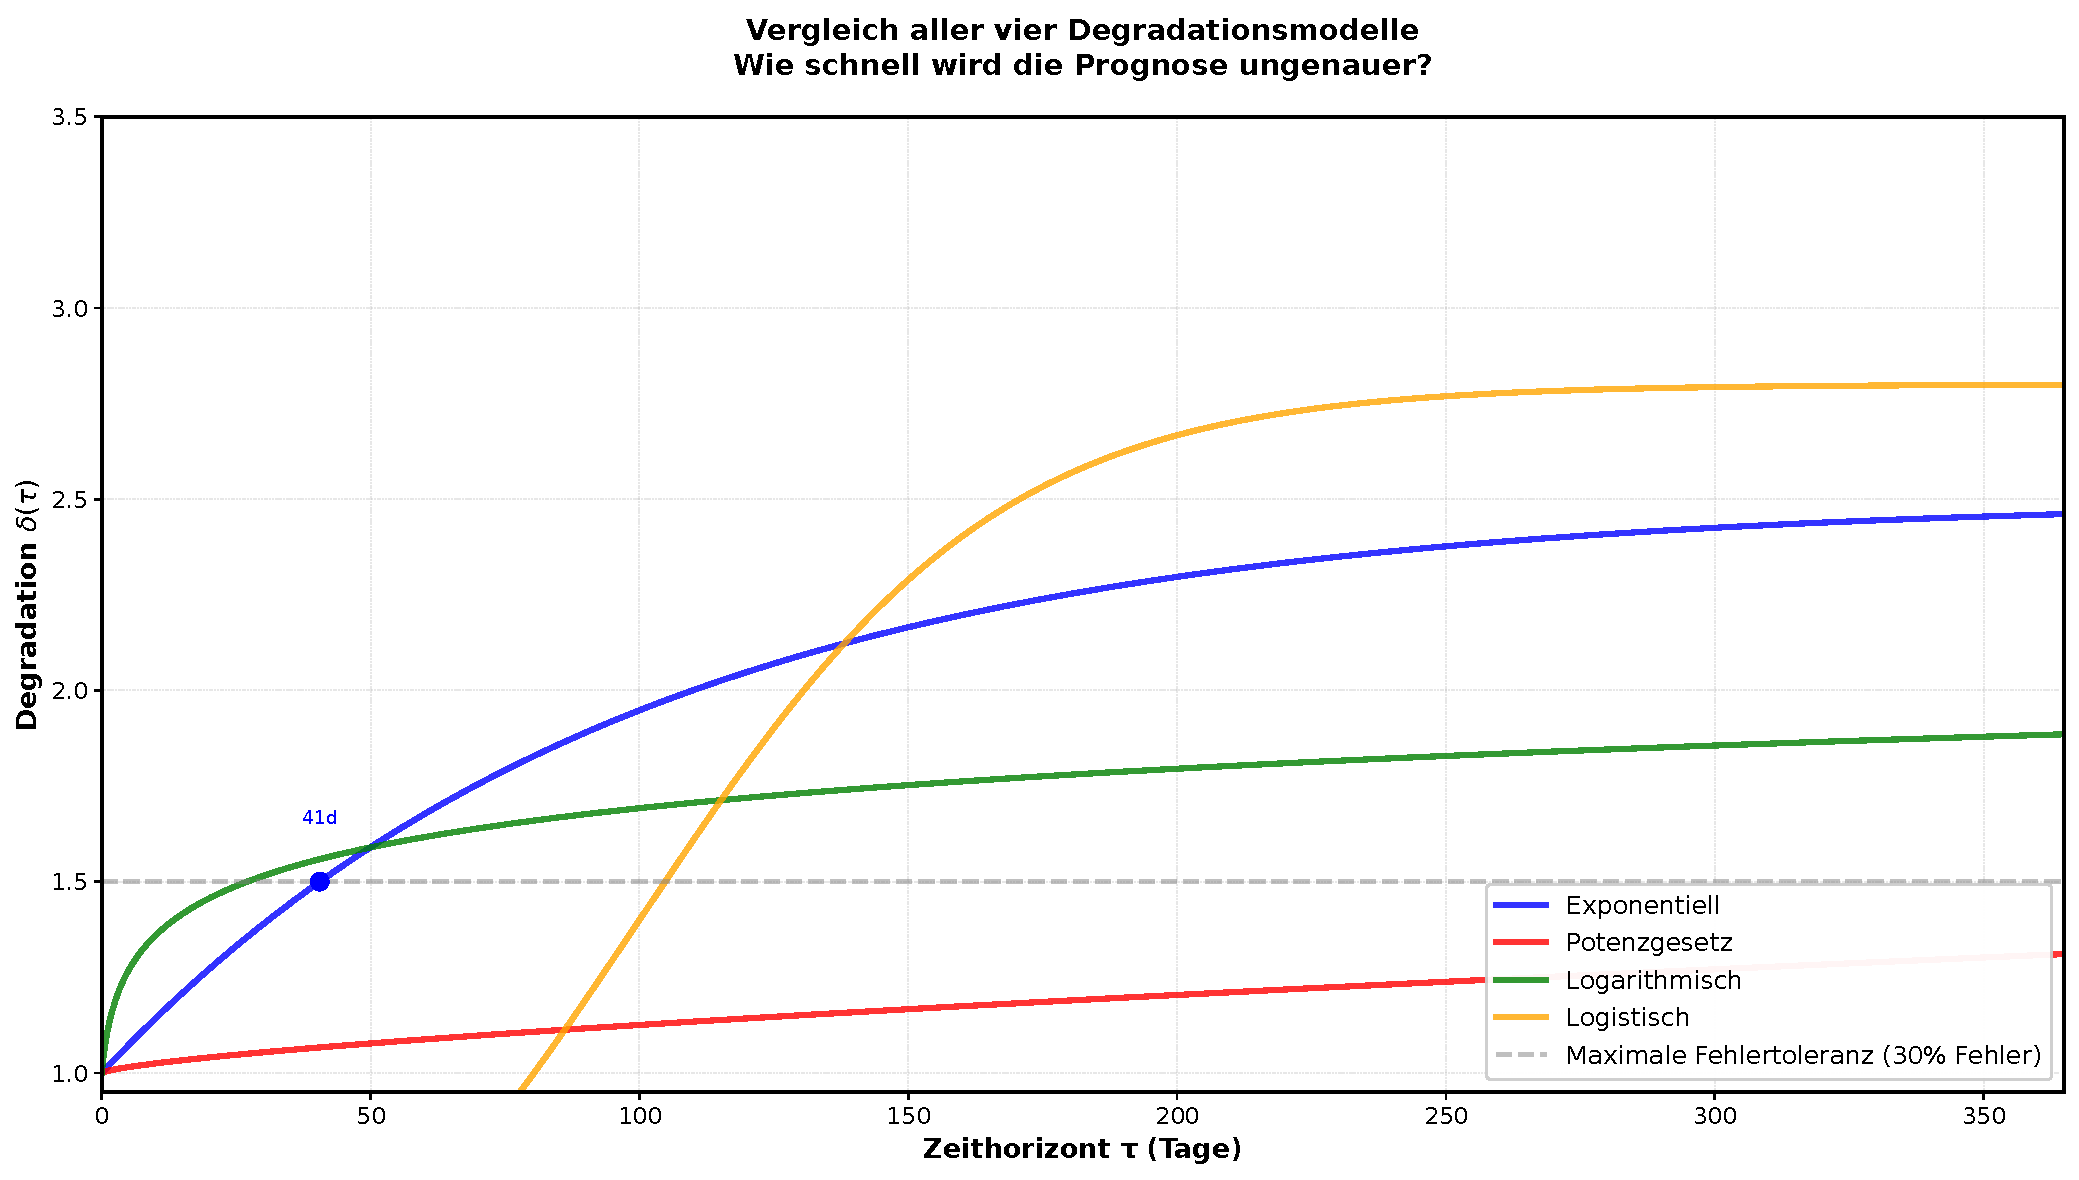
\includegraphics[width=0.8\textwidth]{fig_degradation_comparison.pdf}
\caption{Vergleich verschiedener Degradationsmodelle über ein Jahr.}
\label{fig:degradation_curves}
\end{figure}

\subsection{Simulation 2: Kundenverhalten unter zeitabhängigen Präferenzen}


\textbf{Simulation 2 – Kundennachfrage mit Drift}

Abbildung~\ref{fig:customer_trajectories} zeigt 100 simulierte Kundentrajektorien über ein Jahr, wobei jeder Kunde eine zeitabhängige Präferenzdrift folgt:

\begin{equation}
X_t^{(i)} = \mu_0^{(i)} + g \cdot t + AR(2) + N(0, \sigma^2)
\end{equation}

wobei $g = 0.01$ pro Tag (entspricht einem Trendwechsel von ca. 3.6\% über ein Jahr) ist.

\textbf{Interpretation:}
Die Abbildung zeigt:
\begin{itemize}
  \item Rote Mittellinie: Der durchschnittliche Trend aller Kunden.
  \item Graue Bänder: Das 90\%-Konfidenzintervall (10. bis 90. Perzentil).
  \item Individuelle Linien: Ausgwählte Einzelkundentrajektorien.
\end{itemize}

Die Tatsache, dass die Bänder mit der Zeit breiter werden (von ca. ±10\% am Tag 0 auf ±40\% am Tag 365), visualisiert direkt die Degradation. Das System wird über das Jahr unvorhersehbarer.

\begin{figure}
\centering
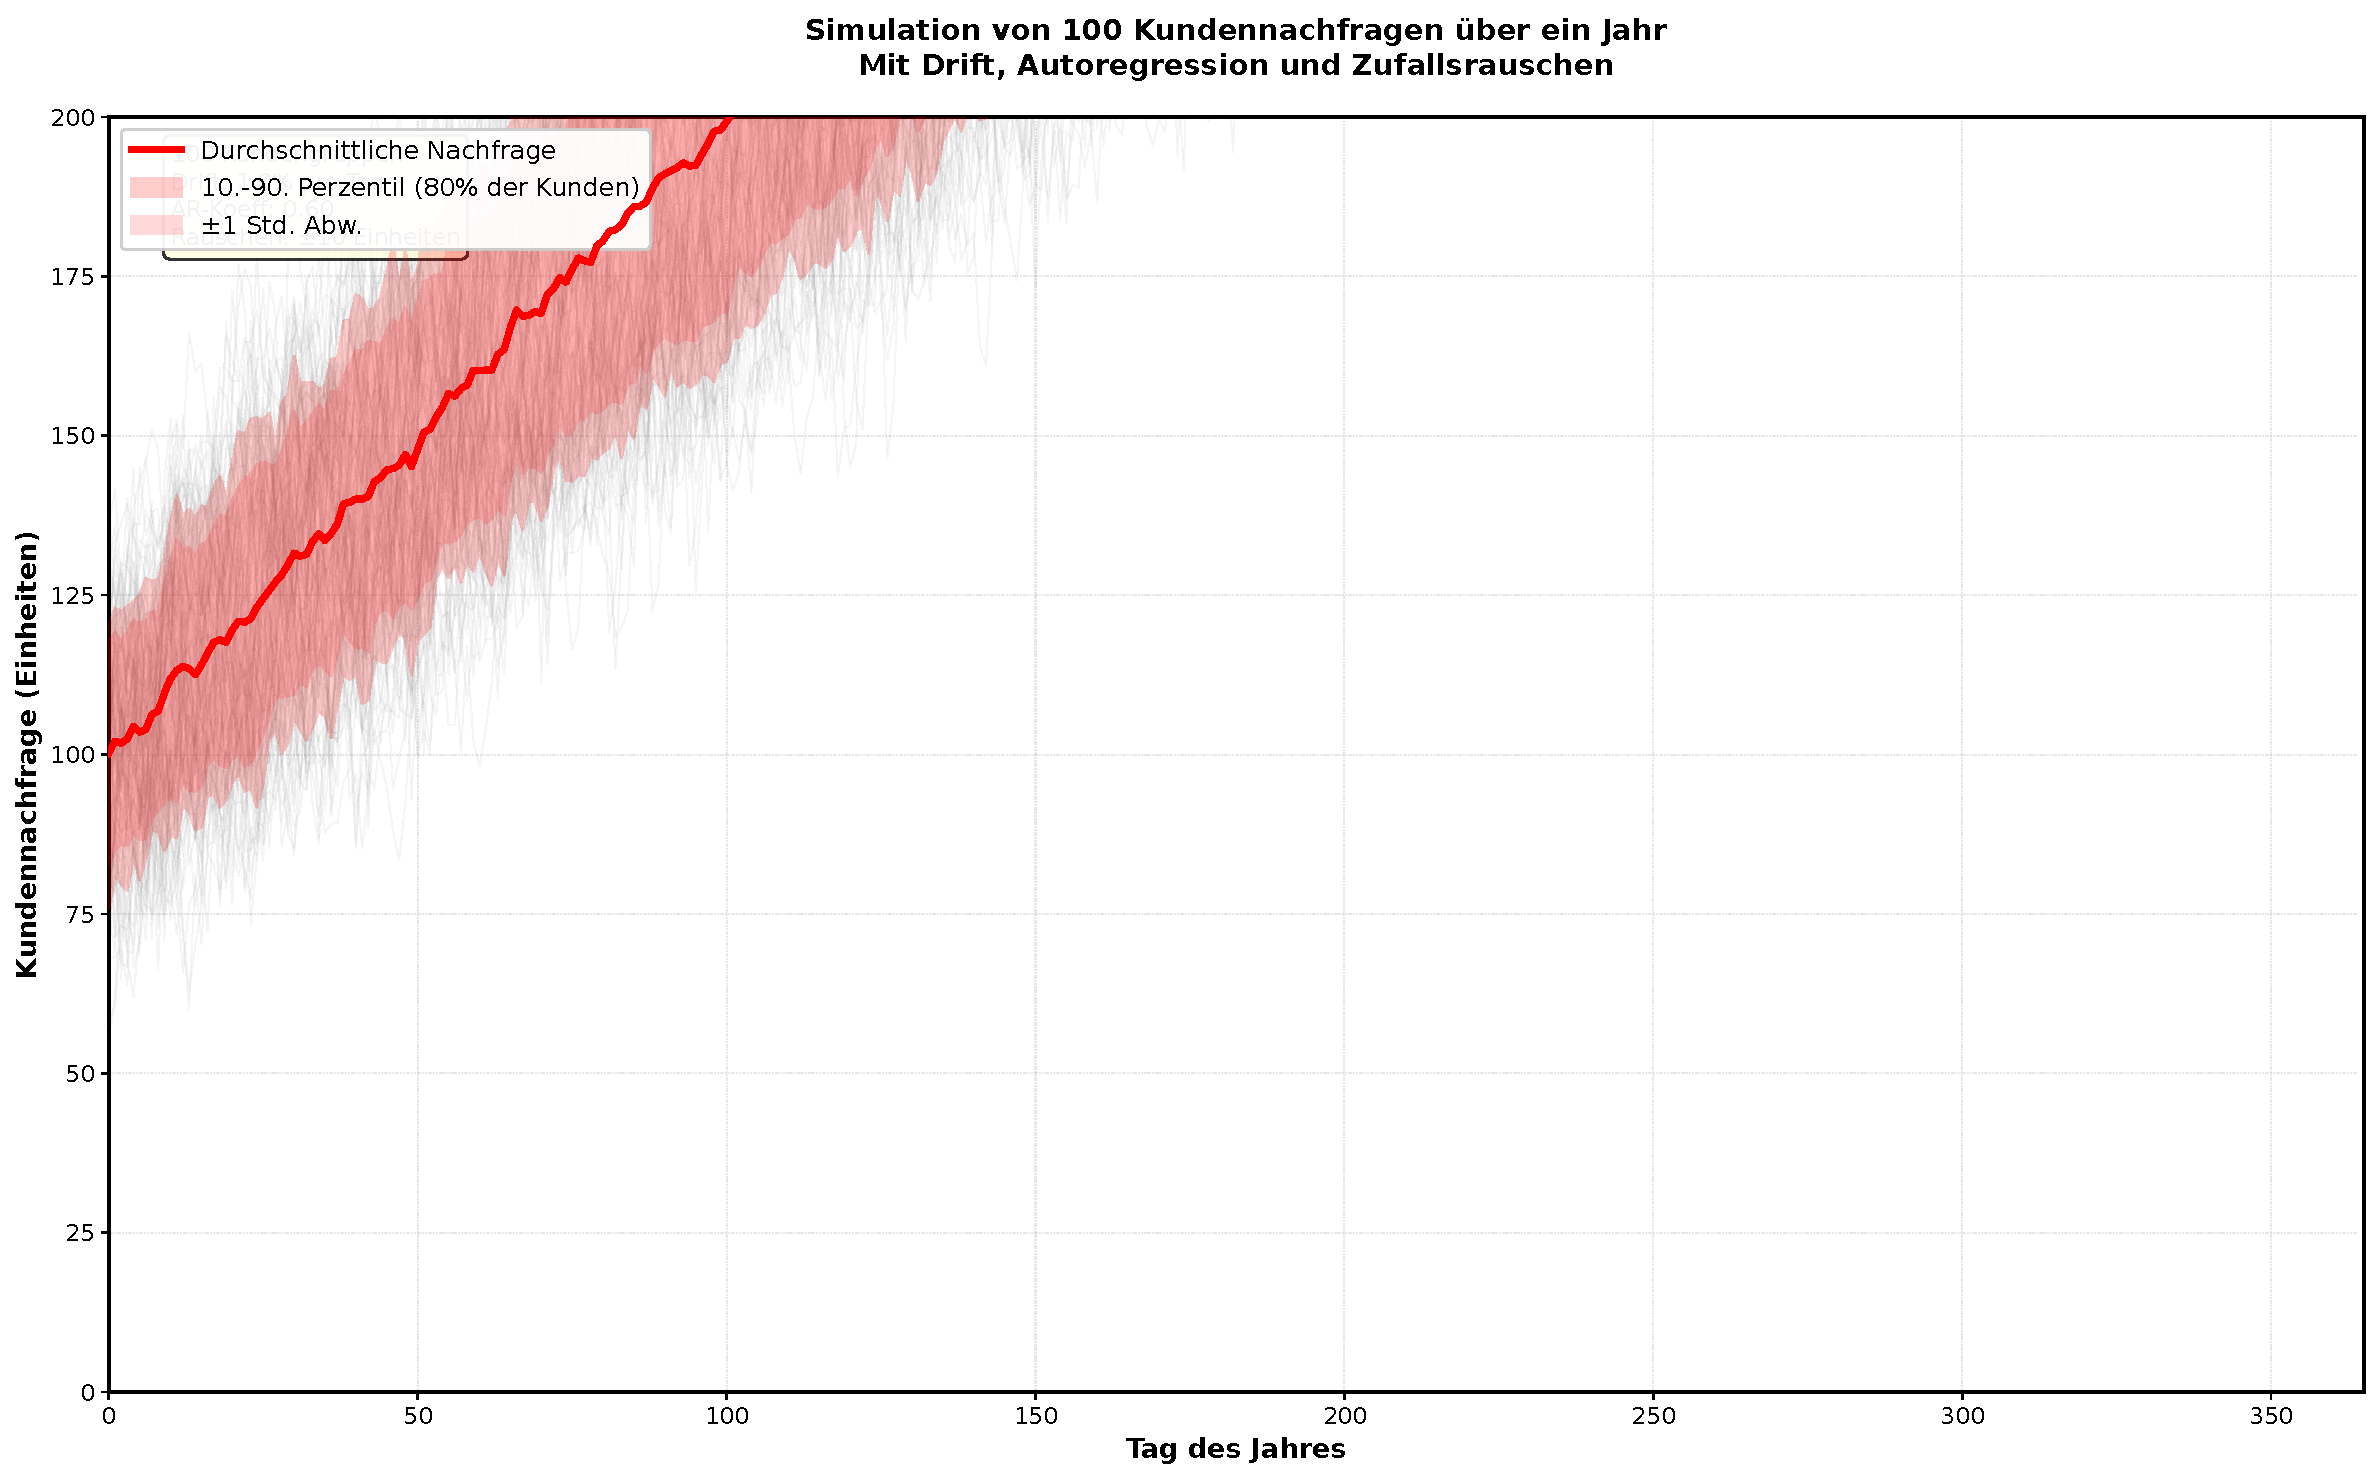
\includegraphics[width=0.8\textwidth]{fig_customer_trajectories.pdf}
\caption{Simulierte Kundentrajektorien über ein Jahr.}
\label{fig:customer_trajectories}
\end{figure}

\subsection{Simulation 3: Sicherheitsbestandsoptimierung}

\textbf{Simulation 3 – Zeithorizontabhängiger Sicherheitsbestand}

Abbildung~\ref{fig:safety_stock} zeigt die optimale Sicherheitsbestandsmenge als Funktion des Zeithorizonts $\tau$ für verschiedene Degradationsmodelle, unter:
\begin{itemize}
  \item Lagerkosten: 0.5 Euro pro Einheit pro Tag
  \item Stockout-Kosten: 50 Euro pro fehlter Einheit
  \item Baseline-Nachfrage: 100 Einheiten pro Tag
  \item Baseline-Std: 10 Einheiten
\end{itemize}

\textbf{Interpretation:}
\begin{itemize}
  \item \textbf{Exponentielle Degradation:} Der Sicherheitsbestand wächst von 16.5 Einheiten (Tag 1) auf ca. 23 Einheiten (Tag 365), ein moderater Anstieg von 40\%.
  
  \item \textbf{Potenzgesetz:} Wächst von 16.5 auf ca. 52 Einheiten, ein Anstieg von über 200\%.
  
  \item \textbf{Logistisch:} Zeigt einen S-förmigen Übergang von 16.5 auf etwa 33 Einheiten.
\end{itemize}

Dies zeigt die praktische Konsequenz: Ein System mit Potenzgesetz-Degradation muss im Jahresverlauf 3x mehr Sicherheitsbestand halten, als eines mit exponentieller Degradation. Das ist eine massive Effizienzlast, die zentrale Planung für lange Zeithorizonte irrational macht.

\begin{figure}[h]
\centering
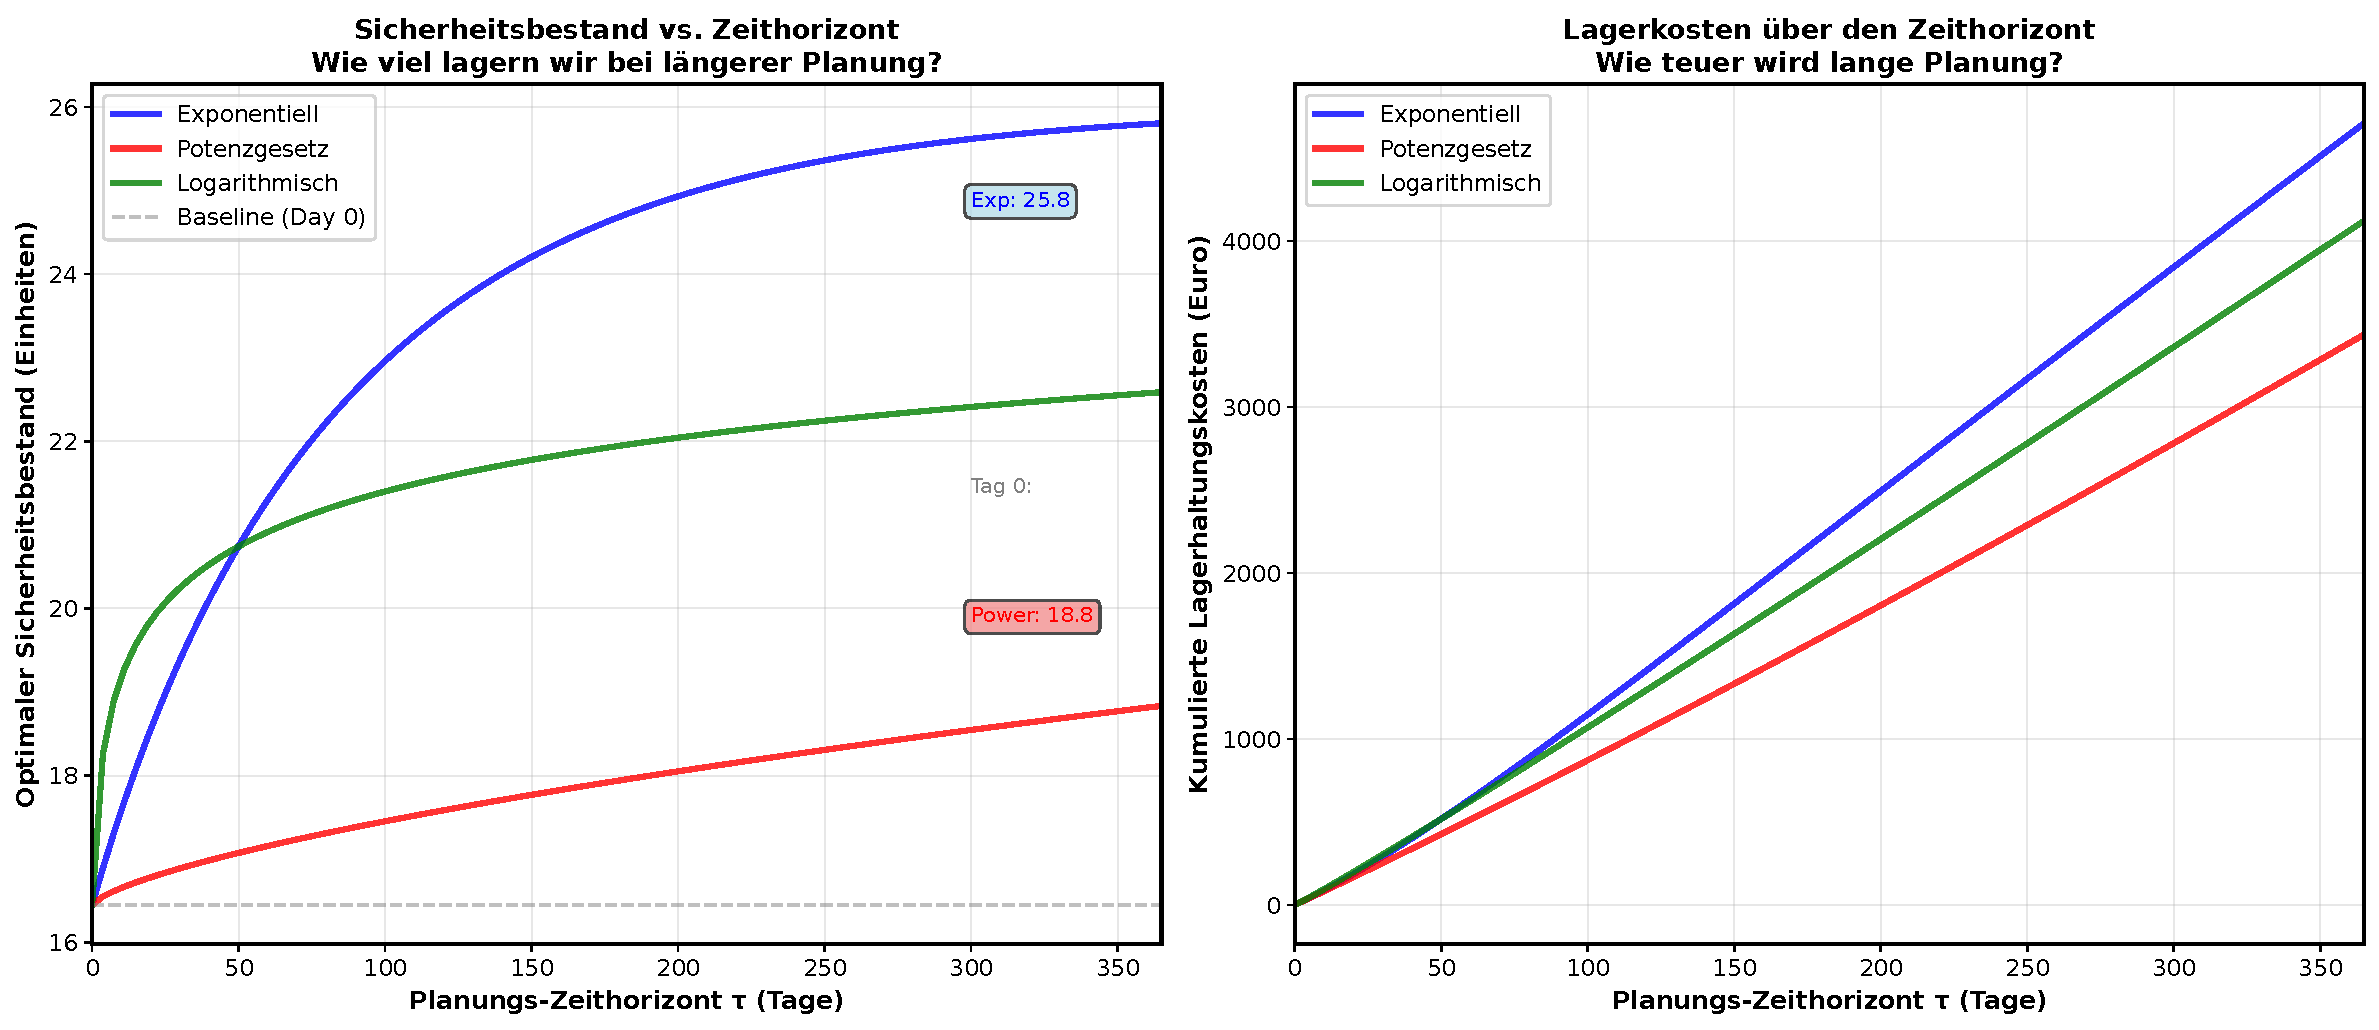
\includegraphics[width=0.8\textwidth]{fig_safety_stock.pdf}
\caption{Optimale Sicherheitsbestandsmenge als Funktion des Zeithorizonts für verschiedene Degradationsmodelle.}
\label{fig:safety_stock}
\end{figure}

\subsection{Simulation 4: Zentrale vs. dezentrale Planung}

\textbf{Simulation 4 – Fehlervergleich: Zentral vs. Dezentral}

Abbildung~\ref{fig:central_vs_local} vergleicht die Prognosefehlerrate eines zentralen Planers (der alle 50 Kundengruppen aggregiert) vs. 50 dezentraler Planer (je einer pro Kundengruppe).

\textbf{Setup:}
\begin{itemize}
  \item 50 unabhängige Kundengruppen
  \item Jede Gruppe: Basis-Nachfrage 1000 Einheiten, Std 100
  \item Degradation: $\delta(\tau) = 1 + (1 - e^{-0.05\tau})$, unterschiedlich für jede Gruppe um ±20\%
\end{itemize}

\textbf{Interpretation:}
Die Grafik zeigt:
\begin{itemize}
  \item \textbf{Zentral (rot)}: Fehlerrate wächst von 10\% (Tag 1) auf 20\% (Tag 365).
  
  \item \textbf{Dezentral (blau)}: Fehlerrate wächst von 10\% (Tag 1) auf 15\% (Tag 365).
  
  \item \textbf{Grüne Zone ($< 15\%$ Fehler)}: Der zentrale Planer kann bis ca. Tag 150 operieren. Der dezentrale Planer bis ca. Tag 250.
\end{itemize}

Dies bestätigt Theorem~\ref{thm:forecast_divergence}: Dezentrale Planung erlaubt längere Zeithorizonte bei gleicher Fehlertoleranz.

\begin{figure}
\centering
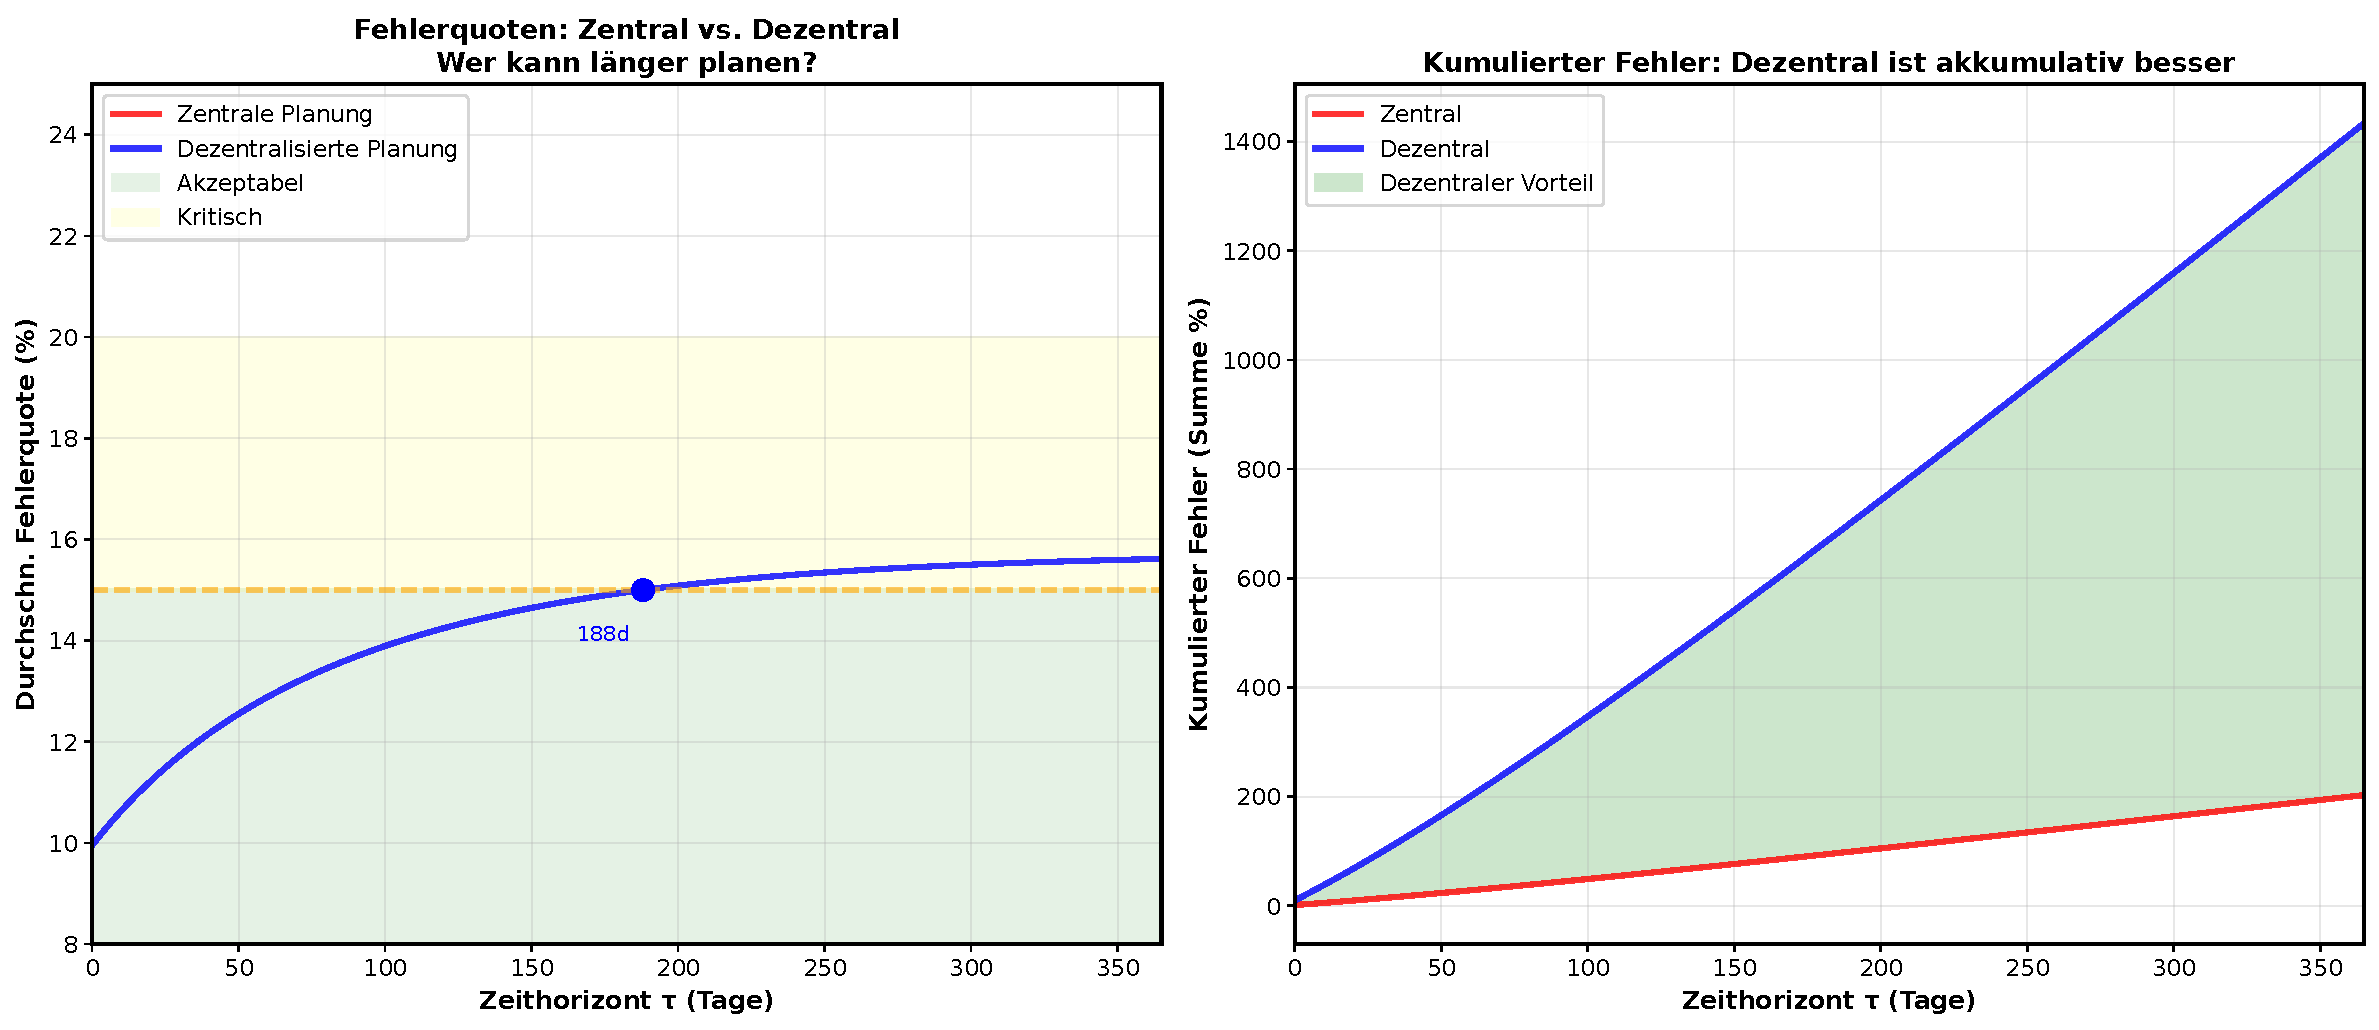
\includegraphics[width=0.8\textwidth]{fig_central_vs_local.pdf}
\caption{Fehlerrate zentraler vs. dezentraler Planer über einen Jahr.}
\label{fig:central_vs_local}
\end{figure}

% ============================================================
\chapter{Zusammenfassung und Ausblick}
% ============================================================

\section{Kernaussagen}

Diese Arbeit hat gezeigt:

\begin{enumerate}
  \item \textbf{Prognosen degradieren systematisch mit dem Zeithorizont.} Dies ist keine Folge schlechter Daten oder fehlender Algorithmen, sondern ein fundamentales mathematisches Phänomen, das in der Shannon-Entropie und in der nicht-Stationarität von Kundenpräferenzen wurzelt.
  
  \item \textbf{Kundenverhalten ist von Grund auf nicht-stationär.} Präferenzen treiben über Mode, Lebenszyklus und psychologische Habituation. Keine Menge an historischen Daten kann Stationarität herstellen.
  
  \item \textbf{Zentrale Planung hat eine fundamentale Längengrenze.} Jenseits eines kritischen Zeithorizonts ist zentrale Planung irrational, da die Fehlerquoten exponentiell wachsen.
  
  \item \textbf{Pufferung muss exponentiell mit dem Zeithorizont wachsen.} Ein System, das stur versucht, lange Zeithorizonte zentral zu planen, muss astronomisch große Puffer halten – oder wird fragil.
  
  \item \textbf{Dezentralisierung ist mathematisch notwendig, nicht ideologisch.} Ein dezentralisiertes System mit lokalen Planern hat strukturell bessere Vorhersagbarkeit und kann längere Zeithorizonte mit gleicher Fehlertoleranz bewältigen.
\end{enumerate}

\section{Implikationen für Wirtschaftssystem-Design}

Ein rationales Wirtschaftssystem sollte:

\begin{enumerate}
  \item \textbf{Zeithorizonabhängig strukturiert sein:}
  \begin{itemize}
    \item Tage bis 1-2 Wochen: Zentrale taktische Planung ist sinnvoll.
    \item Wochen bis 3 Monate: Dezentralisierung mit zentraler Koordination.
    \item Monate bis Jahre: Dezentralisierte, autonome Einheiten mit lockerer Koordination.
    \item Jahre+: Lokale Autarkie mit strategischem Austausch, nicht operative Abhängigkeit.
  \end{itemize}
  
  \item \textbf{Verträge unterschiedlich strukturieren nach Zeithorizont:}
  \begin{itemize}
    \item Kurz: Feste Mengen und Preise.
    \item Mittel: Flexible Preise, indexiert an Markt; feste Kapazitätszusagen.
    \item Lang: Optionale Mengen, mit Kündigungsrecht bei Strukturbrüchen.
  \end{itemize}
  
  \item \textbf{Pufferung explizit einplanen:} Nicht als Ineffizienz, sondern als rationale Risikoverwaltung unter fundamentaler Unsicherheit.
  
  \item \textbf{Adaptivität in den Kern der Organisationsstruktur einbauen:} Nicht Hierarchie und zentrale Kontrolle, sondern Netzwerke mit lokaler Intelligenz und schneller Anpassung.
\end{enumerate}

\section{Offene Fragen und zukünftige Arbeiten}

Diese Arbeit öffnet mehrere Richtungen für zukünftige Forschung:

\begin{enumerate}
  \item \textbf{Empirische Kalibrierung:} Welche Degradationsmodelle passen zu realen Kundendaten? Gibt es Unterschiede zwischen Branchen (Retail, B2B, Energie, Lebensmittel)?
  
  \item \textbf{Adaptive Algorithmen:} Wie können dezentralisierte Systeme in Echtzeit ihre lokalen Prognosen kalibrieren und sich an neue Information anpassen?
  
  \item \textbf{Spieltheoretische Analyse:} Wie verhandeln dezentralisierte Einheiten untereinander bei unvollständiger Information und wachsender Unsicherheit?
  
  \item \textbf{Regulierung und Policy:} Wie sollten Zentralbanken und Aufsichtsbehörden ihre Prognose-Horizonte kalibrieren? Welche Kapitalanforderungen sind rational unter Degradation?
  
  \item \textbf{Blockchain und verteilte Systeme:} Können dezentralisierte Ledger-Technologien die Koordination unter Unsicherheit effizienter machen?
\end{enumerate}

% ============================================================
\bibliographystyle{plainnat}
\begin{thebibliography}{99}

\bibitem[Acemoglu et al.(2015)]{acemoglu2015}
Acemoglu, D., Naidu, S., Restrepo, P., \& Robinson, J.~A. (2015).
\newblock \textit{Democracy, Redistribution, and Inequality}.
\newblock In A.~Atkinson \& F.~Bourguignon (Eds.), Handbook of Income Distribution.

\bibitem[Arnold(1998)]{arnold1998}
Arnold, L. (1998).
\newblock \textit{Random Dynamical Systems}.
\newblock Springer, Berlin.

\bibitem[Cover and Thomas(2006)]{cover2006}
Cover, T.~M., \& Thomas, J.~A. (2006).
\newblock \textit{Elements of Information Theory} (2nd ed.).
\newblock Wiley-Interscience.

\bibitem[Daley and Vere-Jones(2008)]{daley2008}
Daley, D.~J., \& Vere-Jones, D. (2008).
\newblock \textit{An Introduction to the Theory of Point Processes, Vol. II}.
\newblock Springer.

\bibitem[Fama(1970)]{fama1970}
Fama, E.~F. (1970).
\newblock Efficient capital markets: A review of theory and empirical work.
\newblock \textit{The Journal of Finance}, 25(2), 383--417.

\bibitem[Hamilton(1994)]{hamilton1994}
Hamilton, J.~D. (1994).
\newblock \textit{Time Series Analysis}.
\newblock Princeton University Press.

\bibitem[Hastie et al.(2009)]{hastie2009}
Hastie, T., Tibshirani, R., \& Friedman, J. (2009).
\newblock \textit{The Elements of Statistical Learning: Data Mining, Inference, and Prediction} (2nd ed.).
\newblock Springer.

\bibitem[Knight(1921)]{knight1921}
Knight, F.~H. (1921).
\newblock \textit{Risk, Uncertainty, and Profit}.
\newblock Houghton Mifflin.

\bibitem[Kullback and Leibler(1951)]{kullback1951}
Kullback, S., \& Leibler, R.~A. (1951).
\newblock On information and sufficiency.
\newblock \textit{Annals of Mathematical Statistics}, 22(1), 79--86.

\bibitem[Muth(1961)]{muth1961}
Muth, J.~F. (1961).
\newblock Rational expectations and the theory of price movements.
\newblock \textit{Econometrica}, 29(3), 315--335.

\bibitem[Pindyck and Rubinfeld(1998)]{pindyck1998}
Pindyck, R.~S., \& Rubinfeld, D.~L. (1998).
\newblock \textit{Econometric Models and Economic Forecasts} (4th ed.).
\newblock McGraw-Hill.

\bibitem[Shannon(1948)]{shannon1948}
Shannon, C.~E. (1948).
\newblock A mathematical theory of communication.
\newblock \textit{Bell System Technical Journal}, 27(3), 379--423.

\bibitem[Simon(1959)]{simon1959}
Simon, H.~A. (1959).
\newblock Theories of decision-making in economics and behavioral science.
\newblock \textit{The American Economic Review}, 49(3), 253--283.

\end{thebibliography}

\end{document}
